\documentclass[12pt]{article}
\usepackage[margin=1in]{geometry}
\usepackage{amsmath, amssymb}
\usepackage{graphicx}
\usepackage{booktabs}
\usepackage{float}
\usepackage{hyperref}
\usepackage{caption}
\usepackage{setspace}
\usepackage{natbib}
\usepackage{amsmath, amssymb}
\usepackage{graphicx}
\usepackage{tikz}
\usepackage{enumitem}
\usepackage{hyperref}
\usepackage[margin=1in]{geometry}
\usepackage{tcolorbox}
\usepackage{pgfplots}
\usepackage{color,soul}
\usepackage{tabularray}
\usepackage{siunitx}
\usepackage{tikz}


\setlength{\parskip}{0.75em}
\setlength{\parindent}{15pt}
\newtcolorbox{mybox}{colback=gray!5, colframe=blue!50, breakable}
\doublespacing

\title{Air Traffic Liberalization and Consumer Welfare: \\ A Volume-Based Analysis of the 2018 U.S.--Brazil Open Skies Agreement}
\author{Lennard Pische \\ ECON 970: Economics of Trade Policy \\ Dr. Thomas Baranga}
\date{May 7th, 2025}

\begin{document}
\maketitle

\begin{abstract}
\noindent
This paper evaluates the impact of the 2018 Open Skies agreement between the United States and Brazil on international passenger volumes. Using a difference-in-differences design and route-level data from the U.S. Bureau of Transportation Statistics, this study identifies whether liberalization led to an increase in passenger flows, which is interpreted as a proxy for consumer welfare. The paper accounts for concurrent macroeconomic shocks, (notably, Brazil's 2019 recession) and explores the limitations of the model in estimating policy effects. Results suggest a modest short-run traffic increase in 2018, which later fades amid worsening economic conditions.
\end{abstract}

\newpage

\tableofcontents

\newpage

\section{Introduction}
Whether trade liberalization has positive effects on public welfare has long been debated. Economists worldwide regularly conduct studies on prominent trade agreements that seek to liberalize commerce flows between countries, most often concluding that free trade is beneficial for welfare. One important category of such agreements involves international aviation, where Open Skies treaties seek to liberalize air services by removing government-imposed limits on routes, capacity, and pricing. 

However, the exact impact of these agreements drastically varies by context, with specific provisions and market conditions imposed for different Open Skies Agreements (OSAs). In a highly oligopolistic industry such as aviation, states often have vested interests in protecting domestic carriers, which can influence route allocation and policy enforcement. As a result, the impacts of OSAs are rarely uniform. For instance, an OSA might remove bilateral constraints on the number of flights or designated carriers allowed to operate between any two countries, could retain national airline preference for some routes, or could provide full code-share privileges to companies headquartered in different countries. Additionally, even after ratification, airlines typically still have discretion over aircraft size and frequency, individually determining air traffic trends.

In this context, traditional welfare analysis often focuses on airfare reductions to assess how consumers and producers are affected as a result of these agreements. This article, on the other hand, shifts the focus to a quantity-based metric as a proxy for consumer welfare. The core assumption in this model is that higher passenger flows reflect increased consumer benefits --- that is, on average, net positive welfare effects. By exploiting this assumption, this paper can make use of more readily available data on passenger traffic to evaluate the results of open skies agreements (OSAs) rather than having to rely on harder-to-access and often confidential airfare data. Whether OSAs result in measurable increases in traffic volumes, and thus in consumer welfare, consequently becomes an empirical question.

To explore this, the paper examines the U.S.–Brazil Open Skies Agreement, ratified in March 2018 \footnote{Reuters, “Brazil Senate Approves Open Skies Air Deal with United States,” \textit{Reuters}, March 7, 2018, \url{https://www.reuters.com/article/business/brazil-senate-approves-open-skies-air-deal-with-united-states-idUSKCN1GJ2ZG}.}, to examine how traffic between the two countries was affected post-agreement. This OSA removed restrictions on pricing flights between the United States and Brazil, provided ``full code-share rights" and ``additional charter flexibility" to U.S. and Brazil-based airlines, which spurred widespread anticipation of increased traffic flows between the two countries. \footnote{U.S. Department of Transportation, “United States, Brazil Reach Open-Skies Aviation Agreement,” August 1, 2019, \url{https://www.transportation.gov/briefing-room/united-states-brazil-reach-open-skies-aviation-agreement}.} In fact, prior to the OSA ratification, designated carriers from each country were restricted in frequency and routing, and approvals were often negotiated bilaterally --- all of which contributed to instability in traffic volumes.

Using panel data from 2015 to 2020, this paper sets up a difference-in-difference (DiD) empirical framework, using Bureau of Transportation Statistics (BTS) data on international flights originating or arriving on U.S. soil in the sample period. Treated (U.S.-Brazil flights) and control routes (flights from/to the rest of the world) passenger flows are analyzed pre- and post-March 2018, when U.S.-Brazil OSA was ratified. Building on prior literature, this study extends existing analyses by incorporating market fundamentals from the CEPII 2022 Gravity dataset, controlling for hemisphere-based seasonality effects through spatial data available in the RStudio documentation, and accounting for time, route and hemisphere-by-month fixed effects in the model it seeks to build.

\section{Background and Literature Review}
Extensive literature has reviewed the effects of air service liberalization on market outcomes. Classic studies on OSAs often find that liberalizing air routes tends to increase competition and reduce airfares, leading to consumer benefits. For example, Winston and Yan (2015) report ``at least \$4 billion" in gains to U.S. travelers generated by OSAs every year, and note that, in the period they analyze, airfares were 9-32\% higher prior to Open Skies implementation.\footnote{Clifford Winston and Jia Yan, “Open Skies: Estimating Travelers’ Benefits from Free Trade in Airline Services,” \textit{American Economic Journal: Economic Policy} 7, no. 2 (2015): 370–414, \url{https://www.brookings.edu/wp-content/uploads/2016/06/Open-Skies-Published.pdf}.} Beyond airfare effects, however, liberalization also impacts quantity outcomes such as capacity offered and overall passenger traffic. Bernardo and Fageda (2017), in a DiD study of the EU-Morocco OSA, found a ``20-35\% increase in the number of seats offered" on existing routes after the agreement, along with a notable number of new routes launched.\footnote{Valeria Bernardo and Xavier Fageda, “The effects of the Morocco-European Union open skies agreement: A Difference-in-differences analysis,” \textit{Transportation Research Part E: Logistics and Transportation Review, Volume 98, 2017, 24-41} \url{https://doi.org/10.1016/j.tre.2016.11.009}.} OSAs have also been found have increased carrier benefits. For instance, Button (2009) showed that the US–EU OSA generally improved market efficiency and producer (airline) welfare. More specifically, it deepened already-existing global airline alliances, contributed to regional development, helped reduce average costs for the airlines, and created economies of scale, though the author warns that solid antitrust regulation must be in place for these agreements to reach their full potential.\footnote{Kenneth Button, "The Impact of US–EU ‘Open Skies’ Agreement on Airline Market Structures and Airline Networks," \textit{Journal of Air Transport Management} 15, no. 2 (2009): 59–71, \url{https://www.sciencedirect.com/science/article/pii/S0969699708001282}.} 

On the other hand, the literature also notes that outcomes can vary by context. Not all agreements produce immediate traffic surges, as effects might depend on market conditions, airline strategies, and complementary policy. Some highlight that if pre-agreement capacity is not fully utilized or competition is already robust, the incremental effect on traffic of OSAs might be reduced.  Oum et.al (2020), for example, show that the impact of OSAs varies substantially across country pairs. By comparing US and Canada OSAs, they argue that pre-agreement factors such as strong geographical ties, more prohibitive restrictions on travel, and high-demand potential contributed much more to the success of the policy than in country pairs that did not exhibit these conditions. \footnote{Tae H. Oum, Kun Wang, and Jia Yan, “Measuring the Effects of Open Skies Agreements on Bilateral Passenger Flow and Service Trade,” \textit{Transport Policy} 74 (2020): 1–14.} Others show that OSAs may have lagged impacts, where passenger growth materializes a few years after liberalization.\footnote{For example, R. Piermartini and L. Rousová, in \textit{Liberalization of Air Transport Services and Passenger Traffic} (Geneva: World Trade Organization, 2013). The authors analyze data from 184 countries and find that while liberalization generally increases passenger flows, the effects may take several years to materialize, especially where initial market conditions are less favorable.} 

The U.S.–Brazil Open Skies Agreement is particularly relevant in this context, due to its prolonged and politically sensitive gestation period. Negotiations between the two countries began as early as the mid-2000s, but faced significant resistance from Brazilian lawmakers concerned about the competitiveness of their domestic carriers. Additionally, although the treaty was signed in 2011, its ratification in Brazil stalled for several years because of protectionist pressures. It was not until March 2018 that the Brazilian Senate finally ratified the agreement, motivated in part by a broader push for regulatory modernization and international competitiveness in the aviation sector. \footnote{Reuters, “Brazil Senate Approves Open Skies Air Deal with United States,” \textit{Reuters}, March 7, 2018, \url{https://www.reuters.com/article/business/brazil-senate-approves-open-skies-air-deal-with-united-states-idUSKCN1GJ2ZG}.} Thus, the U.S.–Brazil OSA provides an especially valuable case study of a delayed liberalization shock in a major emerging market context.

In summary, then, the literary consensus seems to rest on the fact that air traffic liberalization tends to improve consumer welfare. However, the magnitude of such impact remains an empirical question. In order to compute analyses on consumer welfare effects, prior research has emphasized looking at fare reductions and consumer surplus calculations. My work aligns with such methods, but it slightly pivots from the traditional framework to include passenger quantity as the welfare indicator. By focusing on a recent (post-2018) case, my study also updates the literature with contemporary evidence, accounting for recent industry dynamics (e.g. new market entrants and external shocks like economic fluctuations). This is particularly relevant for policy evaluations when price data are scarce (such as in the analyzed case). The assumption that volume data can reliably signal welfare changes can make my analysis a valuable tool for researchers and regulators.

\section{Data and Sources}

To empirically analyze the impact of the 2018 U.S.-Brazil Open Skies Agreement, I make use of publicly available panel datasets on route-level international air passenger volumes before and after the policy implementation. The main source of non-proprietary data is the U.S. Bureau of Transportation Statistics (BTS). BTS publishes detailed international aviation statistics on an annual basis, divided by flight segment region of interest. 

More specifically, I collect data from the T-100 International Segment Data report on monthly passenger counts on all non-stop flights between U.S. and foreign airports. \footnote{U.S. Bureau of Transportation Statistics, \textit{T-100 International Segment (All Carriers)} dataset. Available at: \url{https://tinyurl.com/BTSdata}.} This dataset includes both U.S. and foreign carriers operating from and to the U.S. every year. For example, BTS records show that in 2019 (just a year after the OSA was ratified), about 241 million passengers flew internationally from and to the U.S. in total. 

To complement this, I then merge this dataset with macroeconomic indicators sourced from the CEPII 2022 Gravity dataset
\footnote{Conte, M., Cotterlaz, P., and Mayer, T. “The CEPII Gravity Database.” CEPII Working Paper No. 2022-05, July 2022. Available at: \url{https://www.cepii.fr/CEPII/en/bdd_modele/bdd_modele_item.asp?id=8}.}(GDP and population by country-year) and use the \texttt{rnaturalearth} \footnote{Philippe Massicotte and Andy South, rnaturalearth: World Map Data from Natural Earth, R package version 1.1.0, 2025, \url{https://docs.ropensci.org/rnaturalearth/}.} package included in the R suite to classify each foreign country as Southern or Northern hemisphere based on its geographic centroid.

Lastly, to create a clean and usable panel for analysis,  I aggregate the data at the country-pair and month level. Specifically, for each month, I sum the total number of passengers (inbound and outbound) flown between the United States and each foreign country. The aggregation step allows me to focus on bilateral passenger flows at a level appropriate for evaluating international policy shocks, rather than being influenced by individual carrier routing decisions or seasonal fluctuations in specific country pairs. The final unit of observation is thus at the $(Country Pair, YearMonth)$ level.

From this aggregated dataset, I construct a balanced panel covering January 2015 to March 2020 (by binding the different yearly datasets together). I then extract route passenger totals for each month starting in 2015 and ending in early 2020 (March 2020 is chosen as the cutoff to avoid the disruptive effects of the COVID-19 pandemic on international air travel). The treatment group consists of the U.S.–Brazil country pair, while the control group includes U.S. routes to all other foreign countries during the same period. 

The final panel contains 4,696 monthly country pair observations, with the key outcome variable in the study being the log of the number of passengers traveling on a given country pair route (e.g., between the U.S. and Brazil) in a given time period. \footnote{Approximately 1,400 observations are excluded due to missing values in country-level variables such as GDP or hemisphere classification. These missing values primarily affect countries with near-zero passenger flows throughout the sample period in the BTS dataset, so they do not pose a significant threat to inference.}

\section{Empirical Strategy}
\subsection{Difference-in-Differences Model}

To identify the causal impact of the 2018 U.S.–Brazil Open Skies Agreement on international passenger volumes, I implement a segmented difference-in-differences (DiD) model using monthly panel data from the aggregated dataset I constructed. Natural logarithms are chosen for some estimators to account for original data skewness.

The core estimation takes the following form:
\begin{mybox}
\begin{center}

$\ln(\texttt{Passengers})_{i,t} = \alpha + \beta_1 \cdot \texttt{TREAT}_{i,t} + \beta_2 \cdot \texttt{TREAT\_RECESSION}_{i,t} + $\\

$+\beta_3 \cdot \texttt{ln\_gdp\_foreign}_{i,t} + \beta_4 \cdot \texttt{ln\_pop\_foreign}_{i,t} + \gamma_i + \delta_t + \lambda_{h,t} + \varepsilon_{i,t}$

\end{center}
\end{mybox}

\noindent where:

\begin{itemize}[leftmargin=*]
\item $\ln$(\texttt{Passengers})$_{i,t}$, the dependent variable, is the natural logarithm of passenger counts between the U.S. and foreign country pair $i$ in month $t$;
\item \texttt{TREAT}$_{i,t}$, the post-treatment indicator, equals 1 if the route is U.S.–Brazil after April 2018, capturing the post-policy treatment period;
\item \texttt{TREAT\_RECESSION}$_{i,t}$ flags Brazil–U.S. routes during August–December 2019, controlling for the recession’s effect by interacting treatment observations with a recession indicator;
\item \texttt{ln\_gdp\_foreign}$_{i,t}$ is the log of the foreign country’s GDP in year $t$, controlling for market size;
\item \texttt{ln\_pop\_foreign}$_{i,t}$ is the log of the foreign country’s population in year $t$, capturing demand-side effects;
\item $\boldsymbol{\gamma}_i$, $\boldsymbol{\delta}_t$, and $\boldsymbol\lambda_{h,t}$ are country-pair, month-year, and hemisphere-by-month (to capture seasonality) fixed effects, respectively.
\end{itemize}

Standard errors are clustered at the country-pair level to account for within-route correlation over time. \footnote{Here, inference is made possible by the presence of a large number of clusters (177). (\url{https://doi.org/10.1162/003355304772839588})}

\subsection{Treatment Group Definition and Identification}

The treatment group consists of all monthly observations on the U.S.–Brazil route between 2015 and early 2020. The control group comprises U.S. routes to foreign countries in the same sample period. 

The identifying assumption in the model is that of parallel trends: that is, without the U.S.-Brazil OSA, passenger volumes would have followed a path similar to other U.S.-foreign routes. Pre-treatment trend visualizations validate this assumption.

\subsection{Addressing Recessions and Enriching the Model}

To isolate the Open Skies policy effect from concurrent macroeconomic events, I control for both the 2019 Brazilian recession, which may have negatively impacted air travel demand, and disregard the data from the COVID-19 pandemic period. The months from August to December 2019 are flagged as recession months using official economic data, and an interaction term $\texttt{TREAT\_RECESSION}_{i,t}$ is included in the regression to account for this shock. To avoid pandemic-related disruptions, the dataset is truncated at March 2020 (thus, the dataset is filtered to include only those observations for which $\texttt{MONTH}_{2020} <$  3). 

Additionally, by enriching the model with gravity controls (foreign GDP and population) and hemisphere-specific seasonal fixed effects, I account for both structural differences in market size and differential seasonal patterns between hemispheres. This reduces omitted variable bias and allows for a cleaner estimation of the policy’s net effect on international passenger traffic.

\subsection{Fixed Effects}

The inclusion of country-pair ($\gamma_i$) and month-year ($\delta_t$) fixed effects ensures that any unobservable time-invariant characteristics of a route (e.g., distance, baseline tourism demand, airline market structure) or common temporal shocks (e.g., oil prices, macroeconomic conditions) are accounted for. 

In addition, the inclusion of interaction fixed effects between the month-year and southern hemisphere indicators ($\lambda_{h,t}$) allows the model to control for hemisphere-specific seasonality. This allows us not to attribute regular seasonal fluctuations in opposite hemispheres to the policy shock.

\section{Regression Results}
With the empirical framework established, I now turn to the results of the segmented DiD estimation. This approach separately identifies the short-run effects of the 2018 U.S.-Brazil OSA while controlling for concurrent and potentially confounding macroeconomic disruptions, most notably the 2019 Brazilian recession. In what follows, I begin by presenting the main regression findings and then assessing the robustness of my results to alternative specifications and potential confounders.

\subsection{Main Findings}
\hyperref[tab:did-results]{Table~\ref*{tab:did-results}} presents the coefficients yielded by the difference-in-differences regression, allowing me to causally intepret the effect of the U.S.–Brazil 2018 Open Skies Agreement on passenger volumes between the two countries. 
The estimated coefficient for \texttt{TREAT} is $0.008$ and thus slightly positive, although it is not statistically significant at conventional levels. This suggests that monthly passenger volumes on U.S.-Brazil routes may have increased by approximately 0.8\% relative to the control group, though the effect is measured with considerable uncertainty, precisely due to the absence of a statistically significant result.  On the other hand, the coefficient on \texttt{TREAT\_RECESSION} is negative ($-0.091$) and statistically significant at the 5\% level, suggesting that the Brazilian recession substantially eroded the initial gains (though weak) observed in 2018. The striking traits of this analysis are the coefficients for \texttt{ln\_gdp\_foreign} and \texttt{ln\_pop\_foreign}. While statistically insignificant, they are negative, which appears counterintuitive --- that is, they indicate that air traffic flows are decreasing in GDP and population. As introduced earlier, however, these results are difficult to interpret, and display large standard errors ($0.841$ and $2.515$ respectively), which imply that GDP and population might not be strong predictors of passenger volumes in this context. 
\begin{table}[H]
\centering
\caption{Difference-in-Differences: Log Passenger Volumes with Gravity Controls}
\label{tab:did-results}
\begin{tabular}{@{}ll@{}}
\toprule
 & Log(Passengers) Specification \\
\midrule
TREAT & \num{0.008} \\
 & (\num{0.112}) \\
TREAT\_RECESSION & \num{-0.091}\textsuperscript{**} \\
 & (\num{0.044}) \\
ln\_gdp\_foreign & \num{-0.398} \\
 & (\num{0.841}) \\
ln\_pop\_foreign & \num{-0.175} \\
 & (\num{2.515}) \\
Num. Obs. & \num{4696} \\
R\textsuperscript{2} & \num{0.951} \\
R\textsuperscript{2} Within & \num{0.001} \\
RMSE & \num{0.87} \\
Std. Errors & by: COUNTRY\_PAIR \\
Fixed Effects: COUNTRY\_PAIR & \checkmark \\
Fixed Effects: YearMonth & \checkmark \\
Fixed Effects: YM\_HEMI\_FE & \checkmark \\
\bottomrule
\end{tabular}
\vspace{0.5em} 
\begin{flushleft}
\footnotesize \textit{Source}: U.S. Bureau of Transportation Statistics (BTS), T-100 International Segment Data.
\end{flushleft}
\end{table}

This pattern is consistent with prior findings by Oum et.al (2020), who argue that the impacts of OSAs are highly dependent on evolving market conditions and external economic shocks. In this case, it appears that liberalization did not contribute to significant gains in passenger flows, and the 2019 economic headwinds in Brazil counteracted any potential growth stimulus provided by the agreement. In summary, while economic results regarding the short-term effects of the policy shock are hard to interpret in a statistically significant manner, they do point towards 
\begin{enumerate}
    \item[(1)]weak, but positive effects of air traffic liberalization, and
    \item[(2)] negative effects of negative macroeconomic shocks 
\end{enumerate} 
on air passenger flows between the U.S. and Brazil.
\subsection{Graphical Evidence}
Figure~\ref{fig:passenger-trends} plots the monthly indexed evolution of passenger volumes between the United States and Brazil (treatment group) and the set of U.S.-foreign country-pairs (control group). Pre-treatment trends between the groups largely exhibit the same pattern of passenger flows, validating the DiD identification strategy. U.S.-Brazil routes display higher volatility likely due to seasonality, but that is acounted for in the inclusion of hemisphere-by-month fixed effects. 

Following the ratification of the Open Skies Agreement in early 2018 (the black line), the U.S.–Brazil routes continue to exhibit neary identical trends relative to the control group, though the data shows a slight increase in passenger flows. It is important to note that this seemingly present divergence between the two groups is not pronounced until later on in the sample period, and it is just by mid-2018 that changes in passenger volumes between the U.S. and Brazil start steering away from the control trajectory. 

The reason for the initial seemingly parallel trends is that the relative magnitude of the policy’s effect on passenger flows was modest. Although a positive shift is detectable, it represents only about a less than $1\%$ change in total U.S.–Brazil passenger traffic from February 2018, rendering the impact relatively small in practical terms. By mid-2019, the divergence in monthly passenger growth between the groups widens even more, and it appears that Brazil’s 2019 recession (the red line) has a less significant effect on passenger flows between the U.S. and Brazil than in the rest of the world. 

The observed visual trends may initially appear to contradict the regression results, as the gap between the treatment and control groups becomes more pronounced over time. However, this divergence is largely driven by seasonal variation in international air travel, which is explicitly accounted for in the regression through the inclusion of hemisphere-by-time fixed effects. Overall, then, the visual evidence reports that while liberalization may have had a (rather weak and/or ambiguos) positive short-run effect on air passenger volumes, macroeconomic conditions moderated its longer-term impact even more.

\begin{figure}
    \centering
    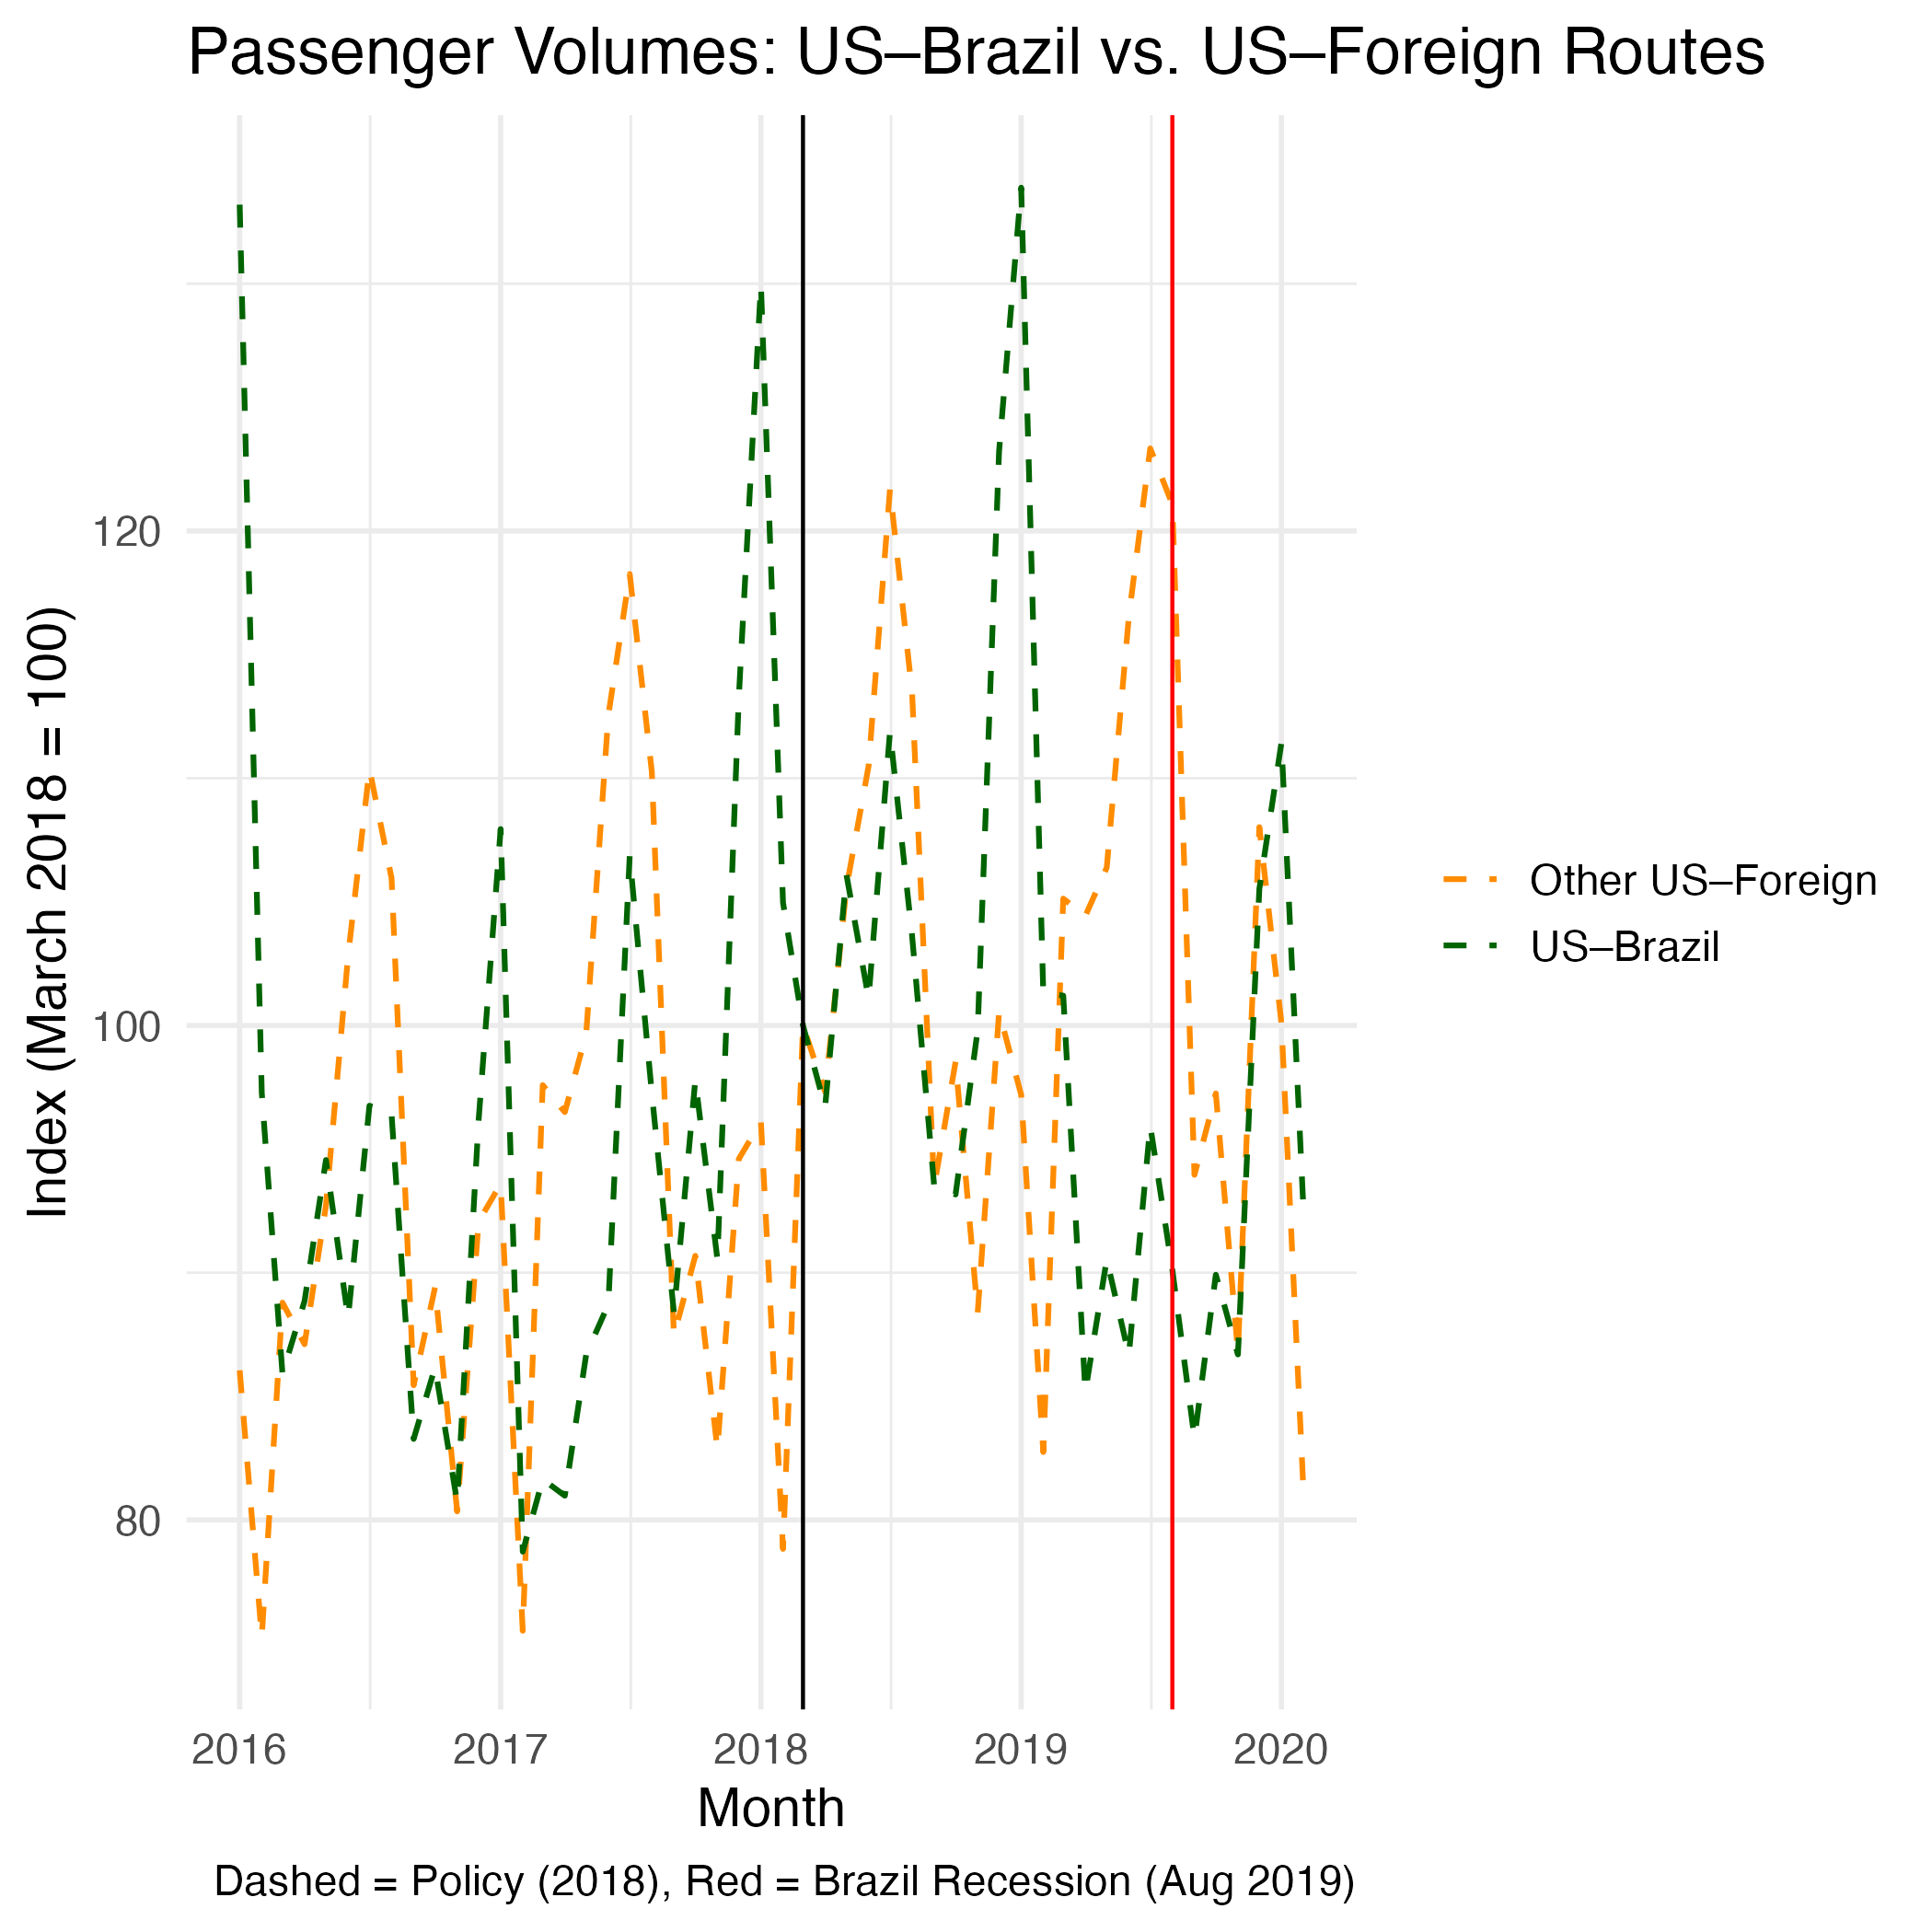
\includegraphics[width=1\linewidth]{us-brazil updates.png} 
\caption{Monthly Passenger Trends on U.S.–Brazil versus U.S.–Latin America Control Routes. Black line indicates OSA implementation (March 2018) and red line indicates onset of Brazilian recession (August 2019).}
    \label{fig:passenger-trends}
    \label{fig:enter-label}
\end{figure}
\subsection{Model limitations}
This design presents some limitations that could pose a threat to general long-term inference, including but not limited to:
\begin{enumerate}
    \item [i.] First, the relatively short post-treatment period before the COVID-19 shock. While data on air transportation volumes is available post-2020, the model would likely need to be modified to control for the effects of the pandemic and other economic shocks, potentially making the model even more difficult to significantly interpret;
    \item [ii.] Second, the relatively small within-R\textsuperscript{2} ($0.001$) and the high value of R\textsuperscript{2} ($0.951$). These values suggests that most variation is absorbed by fixed effects. This is expected given the heavy use of route, time, and hemisphere-by-month fixed effects but still limits precision, as this also means that the model has limited residual variation left to explain and contributes to mostly insignificant coefficient estimates;
    \item [iii.] Third, serial correlation between \texttt{TREAT}and \texttt{TREAT\_RECESSION}. This could confound inference, since the Brazilian recession coincided with part of the post-policy period. To address this, the model separately flags the recession months (August–December 2019). However, perfect separation is not possible, and as a result standard errors are likely increased. Future work could explore instrumental variable methodologies or longer time series to separate these overlapping shocks.
\item[iv.] Lastly, the use of routes to the rest of the world as the control group. While the original model restricted the control sample to a subset of Latin-American countries not subject to an OSA during the sample period, this model chooses the rest of the world as a control group. This serves the model well in providing robust inference (as the cross-sectional sample is larger and made up of 177 country-pairs). However, it may also dilute the validity of the comparison. For example, including high-volume and structurally distinct routes --- such as JFK–LHR (New York to London) --- introduces variation driven by factors unrelated to the U.S.–Brazil routes. As a result, the model’s external validity improves, but its internal comparability to the treatment group may be weakened.
\end{enumerate}

\section{Discussion}
\subsection{Welfare Interpretation}
As introduced earlier in the study, this paper uses quantity-based metrics to develop a welfare-based interpretation of passenger trend shocks after the OSA implementation. Thus, under this framework, any post-March 2018 increase in U.S.–Brazil air passenger volumes can be interpreted as a gain in consumer welfare. This is because, in economic theory, greater availability of air transport services, assuming a flexible prices regime (which the aviation industry in both the U.S. and Latin America, as well as the vast majority of countries in the world, falls into), expands consumer choice and increases consumer surplus. Under a standard demand framework, more flights and more passengers imply that the marginal consumer valuation (of flights) remains higher than or equal to the cost of provision of the service, suggesting net welfare gains. In other words, in a competitive market, an airline will only offer more flights if the amount people are willing to pay (their marginal valuation) is at least as large as the marginal cost of providing that extra seat or flight. However, a consideration must be made: the airline industry is not perfectly competitive, instead displaying the classical traits of oligopolistic markets. This is intuitive, as barriers to entry are high and the market is dominated by a few large carriers. 

Consequently, this paper’s analysis has to slightly pivot from the usual framework of perfect competition. The oligopolistic market structure implies that pricing power, strategic route choices, and government interventions may distort the direct mapping between quantity changes and welfare gains. Nevertheless, even in oligopolistic settings, increases in passenger volumes can still be indicative of welfare improvements, particularly when liberalization reduces regulatory barriers that previously constrained output (i.e., passenger numbers). In the case of OSAs, removing capacity and frequency limits often allows existing carriers to expand services and potentially incentivizes new market entrants, which leads to more competitive dynamics. As a result, air fares might fall, thus leading to higher quantity offered. These prices may not fully adjust to match marginal cost, but this study makes the assumption that any observed increase in quantity still reflects a shift toward a more efficient market equilibrium. \footnote{However, this is only true if the additional demand is voluntary and not artificially inflated by subsidies or protectionist policies.}

Therefore, within this more nuanced framework, passenger growth following the U.S.–Brazil OSA can still be reasonably interpreted as a signal of increased consumer welfare. One consideration to keep in mind when conducting inference is that the precise magnitude of welfare gains might not solely be the result of the OSAs, and could potentially include strategic firm behavior due to the market power each airlines carries in the market.

More generally, aviation liberalization studies  frequently associate traffic increases with welfare improvements. InterVISTAS Consulting (2006), in a landmark study commissioned by the International Air Transport Association (IATA), estimated that liberalizing bilateral air agreements could raise passenger volumes by up to 35\% and boost consumer surplus through increased route availability and reduced travel times. \footnote{InterVISTAS Consulting, \textit{The Economic Impacts of Air Service Liberalization} (Geneva: International Air Transport Association, 2006), available at \url{https://www.iata.org/en/iata-repository/publications/economic-reports/the-economic-impacts-of-air-service-liberalization---intervistas/}.} Similarly, Forsyth (2008) finds that the greater traffic volumes that follow liberalization are associated with gains in consumer welfare. This is due to not only lower fares (which the U.S.-Brazil OSA has likely led to, thanks to the complete removal of pricing restrictions) but also service quality improvements, such as, for example, higher flight frequency and more nonstop connections.\footnote{Peter Forsyth, “The Economic Impact of Air Transport Liberalization,” in \textit{Liberalization in Aviation: Competition, Cooperation and Public Policy}, ed. Kai Hüschelrath, Peter Forsyth, David Gillen, Hans-Martin Niemeier, and Hartmut Wolf (London: Routledge, 2016), 45–62, \url{https://doi.org/10.4324/9781315592305}.}

Altogether, these findings thus validate the choice of using passenger quantity as a reasonable proxy for consumer welfare. Thus, even though direct data on airfares or consumer surplus is unavailable in the chosen datasets, the observed increase in passenger volumes after the U.S.–Brazil Open Skies Agreement could initially seem to support the view that welfare improved in the short run. 

However, it is crucial to recognize that volume increases alone are not always sufficient for sustained welfare gains. As the mentioned authors note, structural reforms like Open Skies must be complemented by competitive airline market structures to avoid outcomes where incumbent airlines capture most of the surplus through monopolistic pricing. The oligopolistic nature of the airline industry makes ensuring reforms crucial for sustained competition and welfare steadiness. As a consequence, due to the small magnitude of the coefficients and hard-to-significantly-interpret regression results, the effect of the OSA can be best characterized as ambiguos. While the initial post-liberalization passenger growth between the U.S. and Brazil is found to have delivered weak, short-term consumer welfare increases, longer-term improvements depend heavily on maintaining robust competition and favorable macroeconomic conditions.

\subsection{Alternative Explanations}

Although the segmented DiD design controls for major shocks like Brazil’s 2019 recession, other confounding factors could partially explain the observed outcomes. 

First, changes in visa regimes — such as the U.S. relaxing visa requirements for Brazilian tourists in mid-2019 — could have independently affected travel demand without being directly tied to the Open Skies agreement (i.e., the effect of the Brazilian recession on air travel could have been understated).\footnote{U.S. Department of State, “Expansion of Interview Waiver Program for Brazilian Nationals,” June 2019, \url{https://br.usembassy.gov/}.} Second, input prices in the aviation industry have been known to undergo a number of fluctuations throughout the years. Global oil price changes between 2018 and 2019 could have altered airline cost structures and route planning, potentially influencing capacity and pricing independent of the policy shock.\footnote{This is potentially captured by time fixed effects, yet it must be addressed as an alternative confounding factor due to its high correlation with distance traveled.} Finally, ongoing airline consolidation (specifically, LATAM Airlines Group's November 2018's joint business agreement with American Airlines) and deeper integration with U.S. carriers may have changed market dynamics through alliance network effects that are hard to isolate from pure OSA effects.

\subsection{Implications for Policy}

The evidence collected from the U.S.–Brazil Open Skies Agreement and the existing literature suggests that, while liberalization can increase consumer welfare through higher passenger volumes, the effects may be modest and fragile without supportive measures.

If the aim is to increase not only consumer welfare as a whole, but also air traffic accessibility, policymakers designing OSAs should complement liberalization with policies that facilitate actual market expansion. For instance, easing visa requirements between partner countries has been shown to significantly boost air travel demand independently of fare reductions.\footnote{InterVISTAS (2006).} Similarly, evidence from the APEC region shows that broader liberalization efforts, including regulatory reforms beyond air services alone, were associated with substantial gains in passenger traffic and trade flows.\footnote{APEC, Liberalisation of Air Services in the APEC Region (1995–2005) (Singapore: Asia-Pacific Economic Cooperation, 2007), \url{https://www.apec.org/docs/default-source/Publications/2007/1/Liberalisation-of-Air-Services-in-the-APEC-Region-19952005-January-2007/07_tpt_airservices.pdf}.} In North America, research reports that liberalization alone is not always sufficient to ensure competitive outcomes, as incumbent carriers have sometimes engaged in predatory practices to exclude new entrants, requiring complementary regulatory oversight to preserve consumer welfare gains.\footnote{Peter Forsyth and David Gillen, eds., \textit{Competition versus Predation in Aviation Markets: A Survey of Experience in North America} (London: Ashgate Publishing, 2010), \url{https://www.taylorfrancis.com/books/edit/10.4324/9781351161404/competition-versus-predation-aviation-markets-peter-forsyth-david-gillen-otto-mayer-hans-martin-niemeier}.}

Low-cost carrier (LCC) entry post-liberalization is also crucial: studies from Gillen and Morrison (2005) show that LCCs can dramatically lower fares and stimulate new travel demand, magnifying the benefits of Open Skies agreements.\footnote{David Gillen and William Morrison, “Regulation, Competition and Network Evolution in Aviation,” \textit{Journal of Air Transport Management} 11, no. 3 (2005): 161–174, \url{https://www.sciencedirect.com/science/article/pii/S096969970500030X}.} Policymakers should thus keep these factors under considerations for new policymaking efforts.

\section{Conclusion and Extensions}

This study examined the effects of the 2018 U.S.–Brazil Open Skies Agreement on international air passenger volumes, using a segmented difference-in-differences framework with fixed effects controls. The findings suggest that liberalization may induce short-term increases in consumer welfare, but that these gains are sensitive to macroeconomic conditions and may dissipate without further supportive policies.

Future research should extend this analysis in at least three directions.

\begin{enumerate}
    \item First, research could incorporate airfare data with the quantity metrics to allow a direct calculation of consumer surplus changes, aligning with the welfare frameworks used in recent air service liberalization studies. Existing fare reduction studies show that, for example, codesharing and airline cooperation, often implicit results of OSAs, are shown to produce fare reductions, which increase consumer surplus. \footnote{Jan K. Brueckner, “International Airfares in the Age of Alliances: The Effects of Codesharing and Antitrust Immunity,” \textit{Review of Economics and Statistics} 85, no. 1 (2003): 105–118, \url{https://doi.org/10.1162/003465303762687749}.} It could thus be beneficial to see both analyses combined.
    \item Second, a deeper investigation into airline entry and exit decisions after OSAs adoption could shed light on whether market structure evolution explains the modest magnitude of the passenger volume gains that the paper observed.
    \item Third, applying the DiD framework to other recent OSAs — such as U.S.–Japan (2010) or EU–ASEAN (2021) — could provide comparative evidence on when and why aviation liberalization succeeds, or not. 
\end{enumerate}  

Exploring these extensions will not only refine our understanding of Open Skies policy impacts but also better inform future global aviation agreements.

\newpage
\bibliographystyle{chicago}
\begin{thebibliography}{}

\bibitem{Reuters2018}
Reuters. "Brazil Senate Approves Open Skies Air Deal with United States." \textit{Reuters}, March 7, 2018. \url{https://www.reuters.com/article/business/brazil-senate-approves-open-skies-air-deal-with-united-states-idUSKCN1GJ2ZG}.

\bibitem{WinstonYan2015}
Winston, Clifford, and Jia Yan. "Open Skies: Estimating Travelers’ Benefits from Free Trade in Airline Services." \textit{American Economic Journal: Economic Policy} 7, no. 2 (2015): 370–414. \url{https://www.brookings.edu/wp-content/uploads/2016/06/Open-Skies-Published.pdf}.

\bibitem{BernardoFageda2017}
Bernardo, Valeria, and Xavier Fageda. "The Effects of the Morocco-European Union Open Skies Agreement: A Difference-in-Differences Analysis." \textit{Transportation Research Part E: Logistics and Transportation Review} 98 (2017): 24–41. \url{https://doi.org/10.1016/j.tre.2016.11.009}.

\bibitem{Button2009}
Button, Kenneth. "The Impact of US–EU 'Open Skies' Agreement on Airline Market Structures and Airline Networks." \textit{Journal of Air Transport Management} 15, no. 2 (2009): 59–71. \url{https://www.sciencedirect.com/science/article/pii/S0969699708001282}.

\bibitem{OumWangYan2020}
Oum, Tae H., Kun Wang, and Jia Yan. "Measuring the Effects of Open Skies Agreements on Bilateral Passenger Flow and Service Trade." \textit{Transport Policy} 74 (2020): 1–14. \url{https://www.sciencedirect.com/science/article/abs/pii/S0967070X18304815}.

\bibitem{PiermartiniRousova2013}
Piermartini, Roberta, and Lucian Cernat Rousová. \textit{Liberalization of Air Transport Services and Passenger Traffic}. Geneva: World Trade Organization, 2013.

\bibitem{BTSdata}
U.S. Bureau of Transportation Statistics. \textit{T-100 International Segment (All Carriers)} dataset. Available at: \url{https://tinyurl.com/BTSdata}.

\bibitem{InterVISTAS2006}
InterVISTAS Consulting. \textit{The Economic Impacts of Air Service Liberalization}. Geneva: International Air Transport Association, 2006. \\
\url{https://www.iata.org/en/iata-repository/publications/economic-reports/the-economic-impacts-of-air-service-liberalization---intervistas/}.

\bibitem{Forsyth2016}
Forsyth, Peter. "The Economic Impact of Air Transport Liberalization." In \textit{Liberalization in Aviation: Competition, Cooperation and Public Policy}, edited by Kai Hüschelrath, Peter Forsyth, David Gillen, Hans-Martin Niemeier, and Hartmut Wolf, 45–62. London: Routledge, 2016. \url{https://doi.org/10.4324/9781315592305}.

\bibitem{StateDept2019}
U.S. Department of State. "Expansion of Interview Waiver Program for Brazilian Nationals." June 2019. \url{https://br.usembassy.gov/}.

\bibitem{APEC2007}
Asia-Pacific Economic Cooperation (APEC). \textit{Liberalisation of Air Services in the APEC Region (1995–2005)}. Singapore: APEC, 2007. \url{https://www.apec.org/docs/default-source/Publications/2007/1/Liberalisation-of-Air-Services-in-the-APEC-Region-19952005-January-2007/07_tpt_airservices.pdf}.

\bibitem{ForsythGillen2010}
Forsyth, Peter, and David Gillen, eds. \textit{Competition versus Predation in Aviation Markets: A Survey of Experience in North America}. London: Ashgate Publishing, 2010. \url{https://www.taylorfrancis.com/books/edit/10.4324/9781351161404/competition-versus-predation-aviation-markets-peter-forsyth-david-gillen-otto-mayer-hans-martin-niemeier}.

\bibitem{GillenMorrison2005}
Gillen, David, and William G. Morrison. "Regulation, Competition and Network Evolution in Aviation." \textit{Journal of Air Transport Management} 11, no. 3 (2005): 161–174. \url{https://www.sciencedirect.com/science/article/pii/S096969970500030X}.

\bibitem{Brueckner2003}
Brueckner, Jan K. "International Airfares in the Age of Alliances: The Effects of Codesharing and Antitrust Immunity." \textit{Review of Economics and Statistics} 85, no. 1 (2003): 105–118. \url{https://doi.org/10.1162/003465303762687749}.

\bibitem{DOT2019}
U.S. Department of Transportation. "United States, Brazil Reach Open-Skies Aviation Agreement." August 1, 2019. \url{https://www.transportation.gov/briefing-room/united-states-brazil-reach-open-skies-aviation-agreement}.

\bibitem{CEPII2022}
Conte, M., Cotterlaz, P., and Mayer, T. "The CEPII Gravity Database." CEPII Working Paper No. 2022-05, July 2022. \url{https://www.cepii.fr/CEPII/en/bdd_modele/bdd_modele_item.asp?id=8}.

\bibitem{rnaturalearth2025}
Massicotte, Philippe, and Andy South. \textit{rnaturalearth: World Map Data from Natural Earth}. R package version 1.1.0, 2025. \url{https://docs.ropensci.org/rnaturalearth/}.

\end{thebibliography}

\end{document}